

%\begin{figure}[b]
%\centering
%\subfigure{\centering 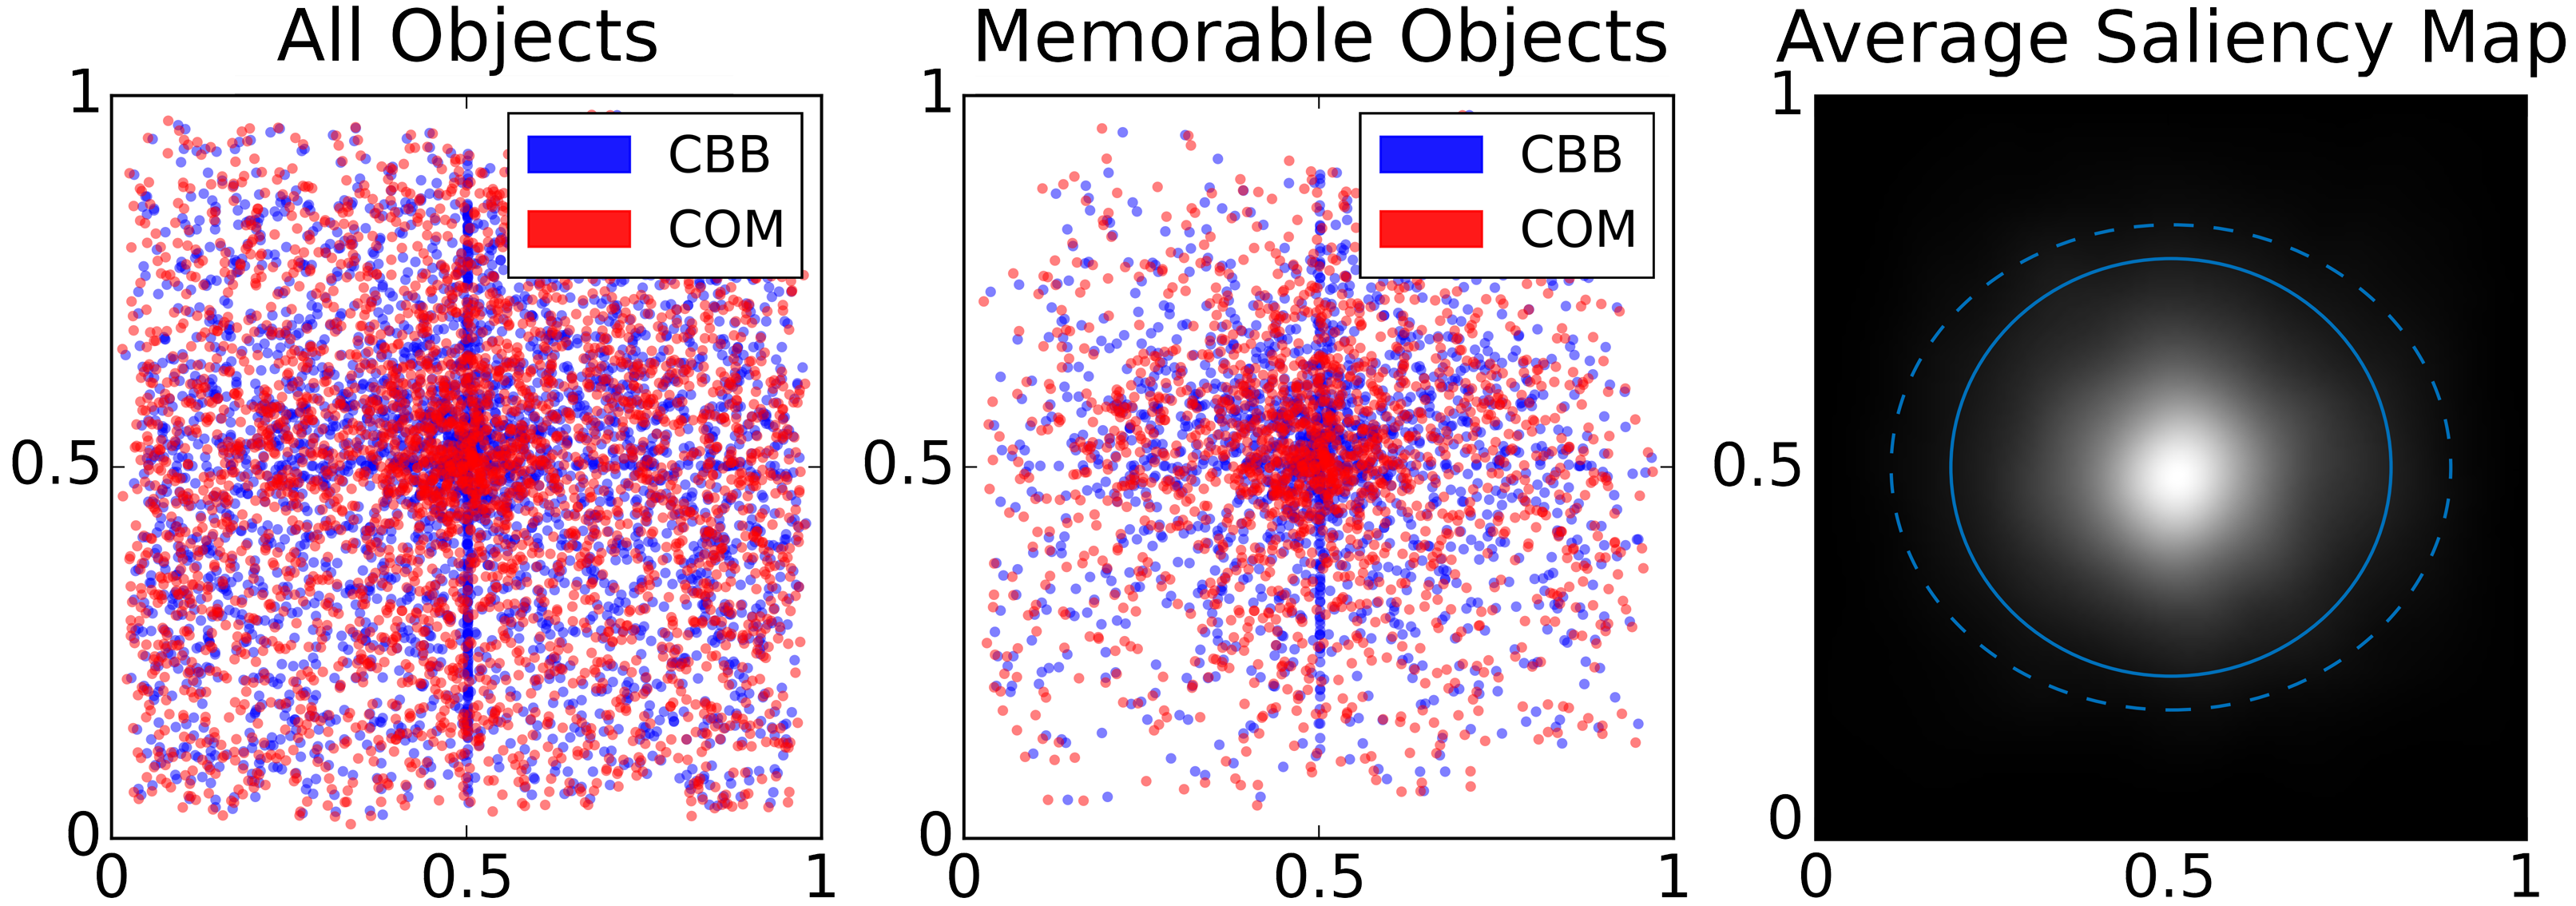
\includegraphics[width=0.5\textwidth]{figures/results/fixation/positions_final.png}}
%\vspace{-5mm}\caption{\footnotesize\textbf{Positions.} add-in later. }\label{fig:exampleStimuli}
%\end{figure}
To examine the relationship between visual saliency and object memorability, we used two indexes of saliency to describe each object. The first was calculated as the number of unique fixation points within the area of each object. The correlation between object memorability and number of fixations within those objects was quite high ($\rho = 0.71$). However, this correlation decreases significantly as the number of total fixations within the object increases. In figure X, we show the correlation between object memorability and number of fixations for subsets of the objects that have at least some minimum number of fixations. On the leftmost side of the plot, the correlation is at it's highest since the set of objects with a fixation count greater than or equal to zero includes all objects and so the correlation is identical to FIGURE FIX-CORR. However, as the minimum number of fixations increases, we look only at objects that contain an increasingly higher number of distinct fixation points, and the correlation decreases. By the time we reach a minimum fixation count of around 35, the correlation falls to around 0.2. This may mean that the predictive value of saliency decreases when there are many areas of interest within a single object. (NOTE: We may want to show examples of images with lots of fixation points that were not well predicted. We could just plot the fixation locations as points on the image) The reason for this decline may be that...[make arguments here] Alternatively, FIGURE Z shows a similar relationship in which the correlation between memorability and fixation count is plotted as a function of minimum number of objects present in the parent image of the object. In a similar pattern, we see that as the minimum number of objects increases, the correlation between fixation count and objet memorability decreases. This follows from the fact that fixation count and number of parent image objects are negatively correlated ($\rho = -0.38$), meaning that if there are more objects in an image, there are less fixation points in any one object, which may a consequence of needing to distribute attention across the objects in the scene. In both scenarios, the ability to predict object memorability sharply decreases.


The second metric we used... (put map method here?)

\begin{figure}[t]
\centering
\subfigure{\centering 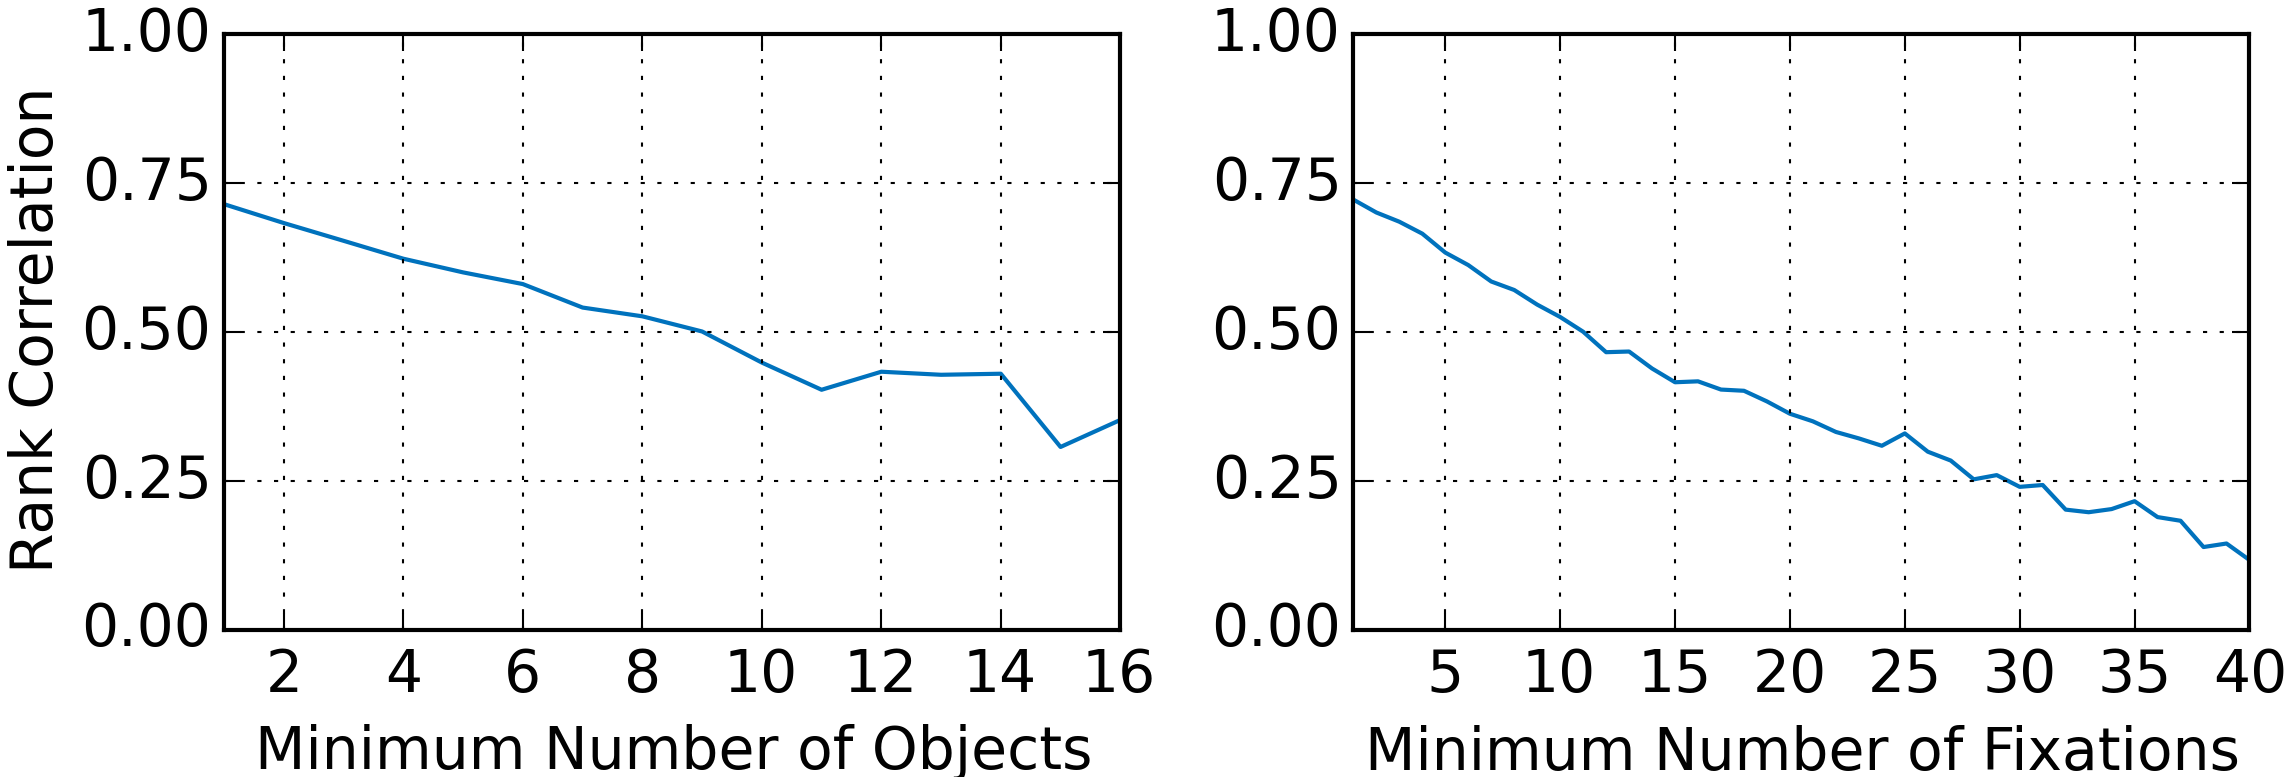
\includegraphics[width=0.5\textwidth]{figures/results/fixation/mem-fix-corr-by-factors.png}}
\vspace{-5mm}\caption{\footnotesize\textbf{Correlation between object memorability and number of fixations.} add-in later. }\label{fig:fixCorr}
\end{figure}


\begin{figure}[b]
\centering
\subfigure{\centering 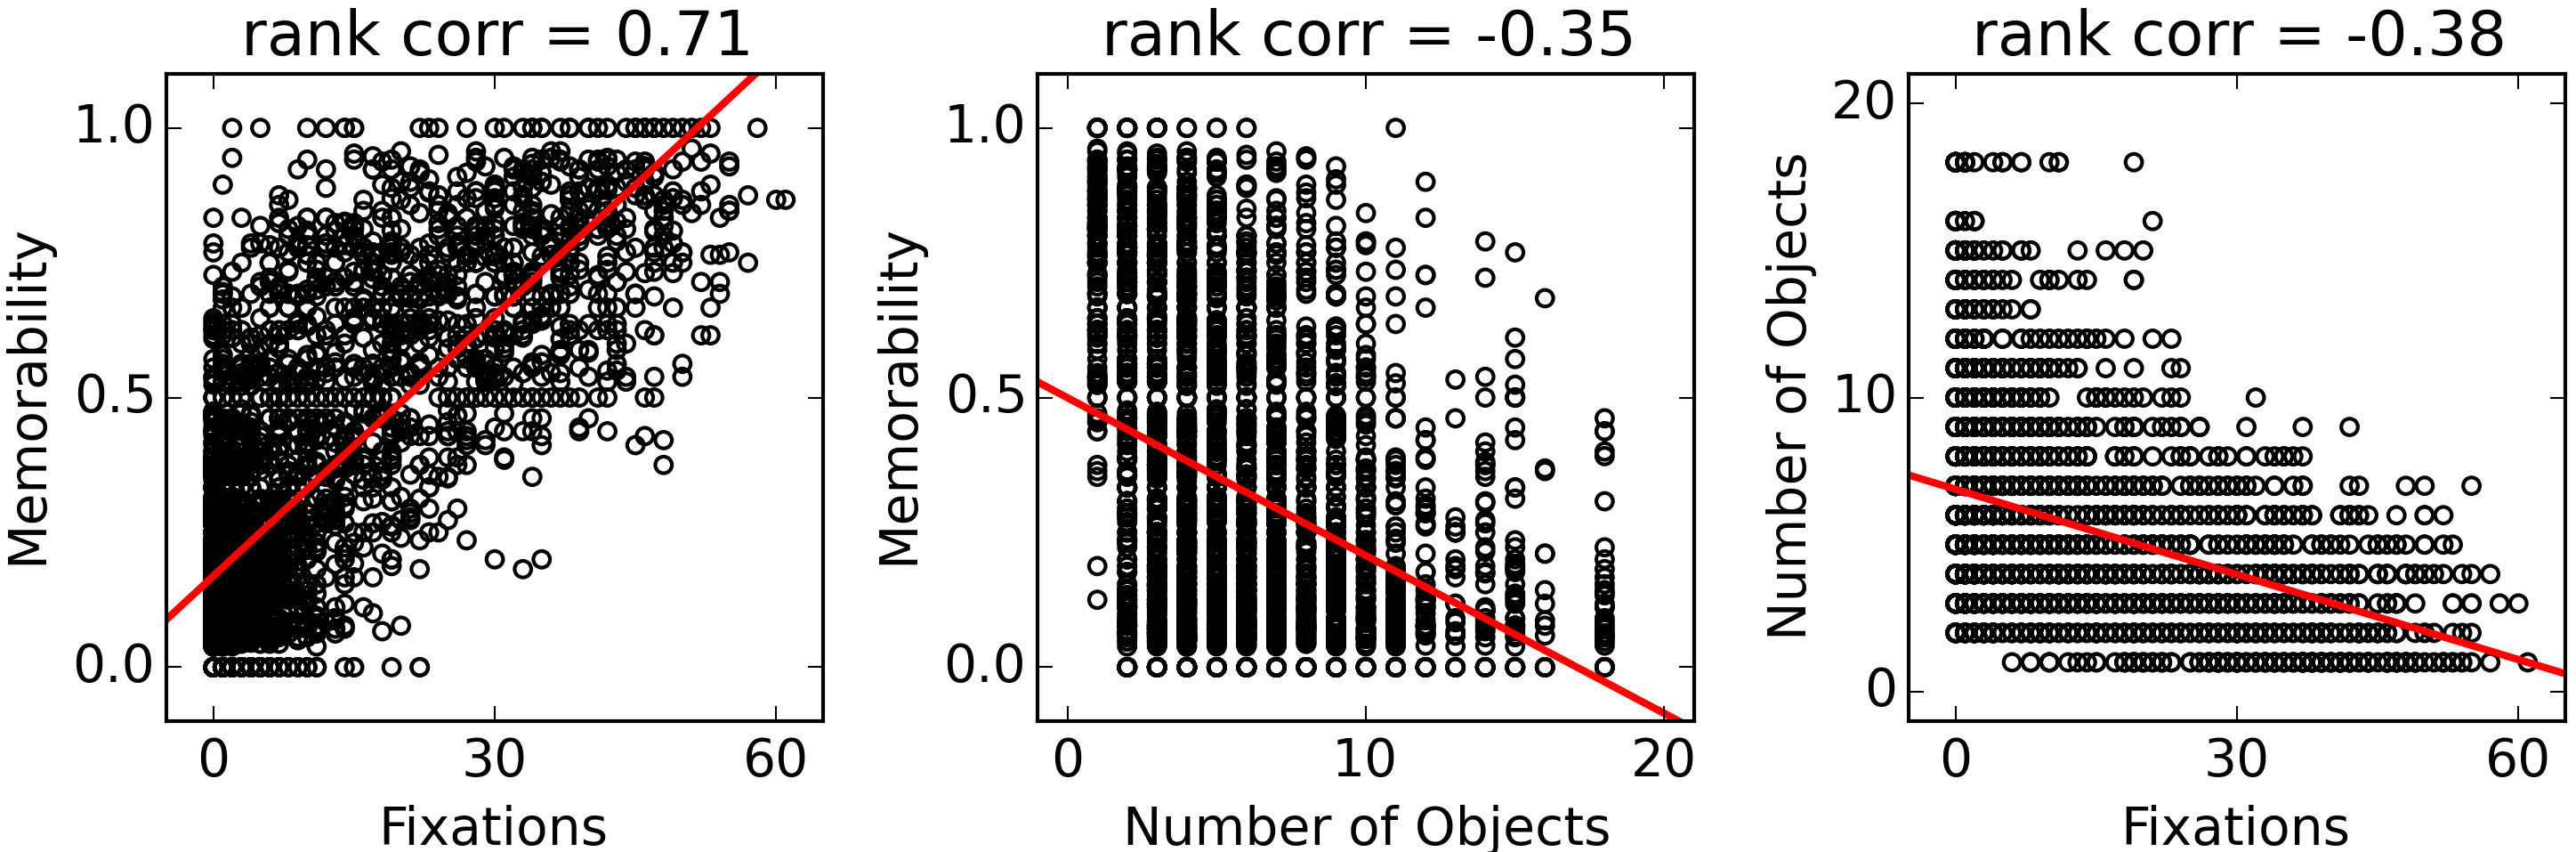
\includegraphics[width=0.5\textwidth]{figures/results/fixation/fix_corr_set.png}}
\vspace{-5mm}\caption{\footnotesize\textbf{Correlation between object memorability and number of fixations.} add-in later. }\label{fig:scatterFixation}
\end{figure}
